\chapter{Introduction}
\label{sec:introduction}

\paragraph{Context.} In recent years, cloud services have become increasingly popular, with many companies moving their technological infrastructure to the cloud. According to Eurostat \cite{eurostat_cloud}, in 2023, 45.2\% of European companies were using cloud services, an increase of 4.2\% compared to 2021. Indeed, major \glspl{csp} like \gls{aws}, Microsoft Azure, and \gls{gcp} now offer a wide range of mature and rich-feature cloud services, with data storage being one of the most commonly entrusted services to the cloud \cite{eurostat_cloud}.
Cloud infrastructures operate on a responsibility-sharing model, where the \gls{csp} and the company collaborate to ensure the security of cloud services. Although specific responsibilities may vary depending on the chosen paradigm (e.g., IaaS, PaaS, and SaaS\footnote{\url{https://www.redhat.com/en/topics/cloud-computing/iaas-vs-paas-vs-saas}}), in general the \gls{csp} is responsible for the protection \textit{of} the cloud, while the company is responsible for the protection \textit{in} the cloud (i.e., the protection of the applications executed and the data stored in the cloud services).
In this context, data breaches become more relevant as the company has no control over the protection of the part of the infrastructure that is the responsibility of the \gls{csp}. In 2022, the Identity Theft Centre reported an alarming 1,774 data breaches, which exposed nearly 400 million user records \cite{itc_2022_databreach}. A data breach can have severe consequences for a company, including financial problems due to compensation and fines, as well as reputational damage \citep{breach_pentagon,breach_verizon,breach_voter}. In Europe, fines may reach up to 4\% of the company's global turnover \cite{eu-gdpr}. 
In addition, \glspl{csp} are generally considered to be honest-but-curious \cite{cac}, meaning that they are assumed to behave correctly when performing the operations entrusted to them (e.g., preserve the integrity of the stored data), but may use the data for other purposes (e.g., advertising, market analysis, AI training). 

For all of the above reasons, protecting data stored in the cloud requires addressing many threats (e.g., external attackers, malicious insiders, honest-but-curious \glspl{csp}) to prevent unauthorized access and ensure confidentiality and integrity. \glspl{csp} often offer a range of data protection and audit mechanisms, such as identity and access management, logs, encrypted disks, and key management. Encryption of data by the \gls{csp} can improve security by mitigating the effects of data breaches or internal threats (e.g., a disloyal employee of the \gls{csp}). However, it is important to note that this is not a definitive solution, as trust in the \glspl{csp} is being shifted from data custody to key custody. In other words, there is the need for a solution that guarantees the protection of data in an honest-but-curious (also called partially trusted) \gls{csp}.

The literature has responded to this need with a wide range of proposals, such as cryptography, steganography, and hardware-based confidential computing. One of these proposals is \gls{cac} --- an approach to \gls{ac} based on full data encryption --- which is diametrically opposed to full trust in \gls{csp}. \gls{cac} require \glspl{csp} to be trusted only for the integrity of resources (usually files), which can be guaranteed by an honest-but-curious \gls{csp}. \gls{cac} is commonly used to protect the confidentiality of sensitive data hosted in the cloud from both external attackers and \gls{csp} itself while enforcing \gls{ac} policies. In \gls{cac}, data is encrypted, and access permissions (such as read access) to the encrypted data are represented by the secret decryption cryptographic keys, which are distributed by a trusted administrator --- e.g., the \gls{it} administrator of the company --- to authorized employees only.


\paragraph{Problem.} Intuitively, \gls{cac} has both advantages and disadvantages. On the one hand, \gls{cac} guarantees confidentiality and data integrity even when the \gls{csp} is honest-but-curious; on the other hand, \gls{cac} requires cryptographic computations that entail a --- often non-negligible --- computational overhead that limits the applicability of \gls{cac} in real-world scenarios. For instance, when an employee is leaving the company, it is essential to regenerate multiple keys and re-encrypt all resources the employee had access to. Otherwise, an employee who previously cached the secret decryption keys could still access data by downloading a resource and decrypting it, possibly colluding with the partially trusted \gls{csp}. While necessary, these cryptographic computations may render \gls{cac} impractical for at least the most dynamic real-world scenarios  \cite{cac}.

Then, we note that \gls{cac} can be used as enforcement mechanism for one of the most widely used \gls{ac} models, i.e., \gls{rbac} \cite{cai_survey_2019}, which includes users, roles, and resources. In brief, a user represents a person, device, or software, while a role represents a job function. Users are assigned to one or more roles, and roles are associated with permissions on resources, allowing for specific operations to be performed. However, assuming a \gls{cac} scheme exists that can dynamically manage security levels based on resource sensitivity, user trust, or other security requirements, \gls{rbac} alone cannot manage such security levels. In fact, \gls{rbac} does not provide suitable abstractions for specifying additional information and constraints that may be useful in reducing the computational overhead of \gls{cac}.
For example, if an employee who is trusted by the administrator is leaving the company, it may not be necessary to regenerate keys and re-encrypt resources.
In addition, in \gls{cac} it is not possible to store public resources, i.e., resources that can be accessed by everyone. Indeed, \gls{cac} expects all resources to be encrypted --- without modification, a completely different process would be necessary to store public files.

In general, all of the previous problems stem from the fact that \gls{cac} typically assumes that the \gls{csp} is not trusted to see the contents of any resource --- the \gls{csp} is only considered trustworthy for the availability and the integrity of resources. Also, \gls{cac} usually assumes that any user would try to access any resource at any time, and that all resources are sensitive. In practice, however, the \glspl{csp} may be trusted to protect some resources, users may have different levels of trustworthiness, and only some resources may be sensitive. For example, if a user loses access to a resource because they have been fired, they may be perceived as less trustworthy. Conversely, if they have been promoted, they may be considered more trustworthy. To the best of our knowledge, no prior solution to those problems has been proposed in the literature.


\paragraph{Solution.} To address the issues mentioned earlier, we propose a new \gls{ac} \erbacwhat that extends \gls{rbac} and allows the company administrator to specify high-level policies that --- according to a specific security model (e.g., defining the levels of trust assumed on users and \glspl{csp}) --- are automatically compiled and enforced by a \hybrid consisting of a \atrcentralized \gls{rbac} enforcement mechanism and \gls{cac} (see \Cref{fig:hybrid}). By defining appropriate formalisms, our \erbac can reduce the computational overhead of cryptographic computations executed in \gls{cac} and enhance its expressiveness. This is achieved by allowing the specification of predicates (i.e., facts about users, roles, resources, and the \gls{csp}) that control the tunable aspects of \gls{cac}; for instance, our \erbac allows to specify the characteristics of entities (e.g., whether a resource should be stored encrypted or unencrypted, whether the \gls{csp} is trusted to protect a resource), the risks of collusion between users and the \glspl{csp}, and the steps to be taken when access is revoked (e.g., whether it is necessary to regenerate keys and re-encrypt resources after revoking access privileges to a user).


\paragraph{Contributions.} In this thesis, we make a number of contributions which we described below:
\begin{itemize}
	
	\item we define an \erbac that allows for specifying predicates defining under what conditions certain cryptographic computations of \gls{cac} should be executed;
	
	\item we define suitable formalisms allowing to automatically compile the \gls{ac} policy specified in the \erbac into two lower-level \gls{ac} policies to be enforced by a centralized \gls{rbac} enforcement mechanism and \gls{cac}, respectively. Moreover, we analyze the computational costs of the cryptographic operations of the resulting \gls{cac} scheme;
	
	\item we implement our \erbac and the formalisms in Prolog to provide a proof-of-concept of our solution.
	
\end{itemize}

\paragraph{Structure.} In \Cref{sec:background}, we explain fundamental concepts of \gls{ac} (\Cref{sec:background.access_control}) and \gls{cac} (\Cref{sec:background.cac}). In \Cref{sec:hybrid}, we provide an overview of the proposed \hybrid (\Cref{sec:hybrid.structure}), examine the \erbac (\Cref{sec:hybrid.scheme}), delve into the \cac (\Cref{sec:hybrid.cac}), and explore cryptographic costs (\Cref{sec:implementation.computation}). \Cref{sec:implementation} presents an implementation of our model, including a list of predicates (\Cref{sec:hybird_istantiation}), an implementation of some components of the \hybrid in Prolog(\Cref{sec:implementation.advanced}), and a concrete demonstration and cryptographic computation analysis of our example (\Cref{sec:implementation.prolog}).


% \Cref{sec:introduction} provides an introduction to our work. \Cref{sec:background} presents the background and related work. In \Cref{sec:hybrid}, we describe our extended model, the modifications made to the CAC model, and our instantiation. Section 4 explains how we implemented the scheme in Prolog and integrated CryptoAC.Finally, Section 5 presents our conclusions. 

% \simonenote{TODO: refs are not clickable }

% \stefanonote{Somewhere in the thesis, I think we could add a graphical representation of our solution to allow the reader understand more easily what we are getting at. More in detail, I think we could add 2 images side-by-side:
	% \begin{itemize}
		% 	\item the first image shows how AC policies are currently enforced with CAC;
		% 	\item the second image shows how AC policies would be enforced with our solution.
		% \end{itemize}
	% Both figures should show what entities are involved (e.g., CryptoAC, cloud provider, administrator) and what is the flow of information (e.g., RBAC policy, data, input/output of each entity). In this way, it is easy for a reader to understand the concrete impact of our solution.
	% I am unsure about the level of details these images should have. It would be useful to place these images here, but of course we cannot rely on notation and symbols that we introduce afterwards in \Cref{sec:background}.
	% }

\begin{figure}[t!]
	\centering
	
	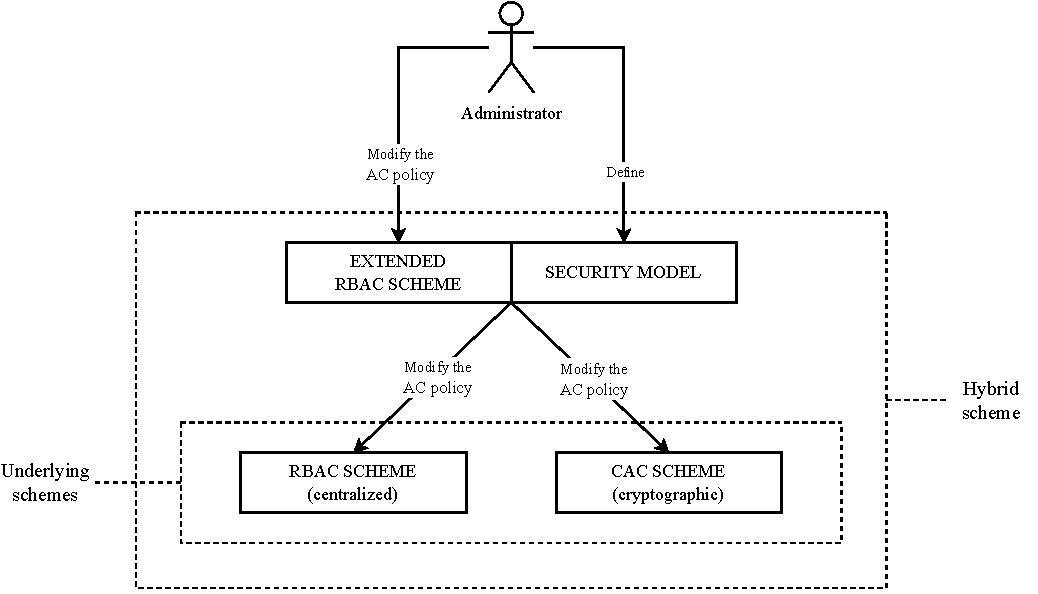
\includegraphics[width=0.85\textwidth]{assets/img2/hybrid.pdf}
	
	\caption{The Hybrid System}
	\label{fig:hybrid}
\end{figure}

% % \begin{figure}[t]
	% % 	\centering
	
	% % 	\begin{subfigure}{0.48\textwidth}
		% % 		\centering
		
		% % 		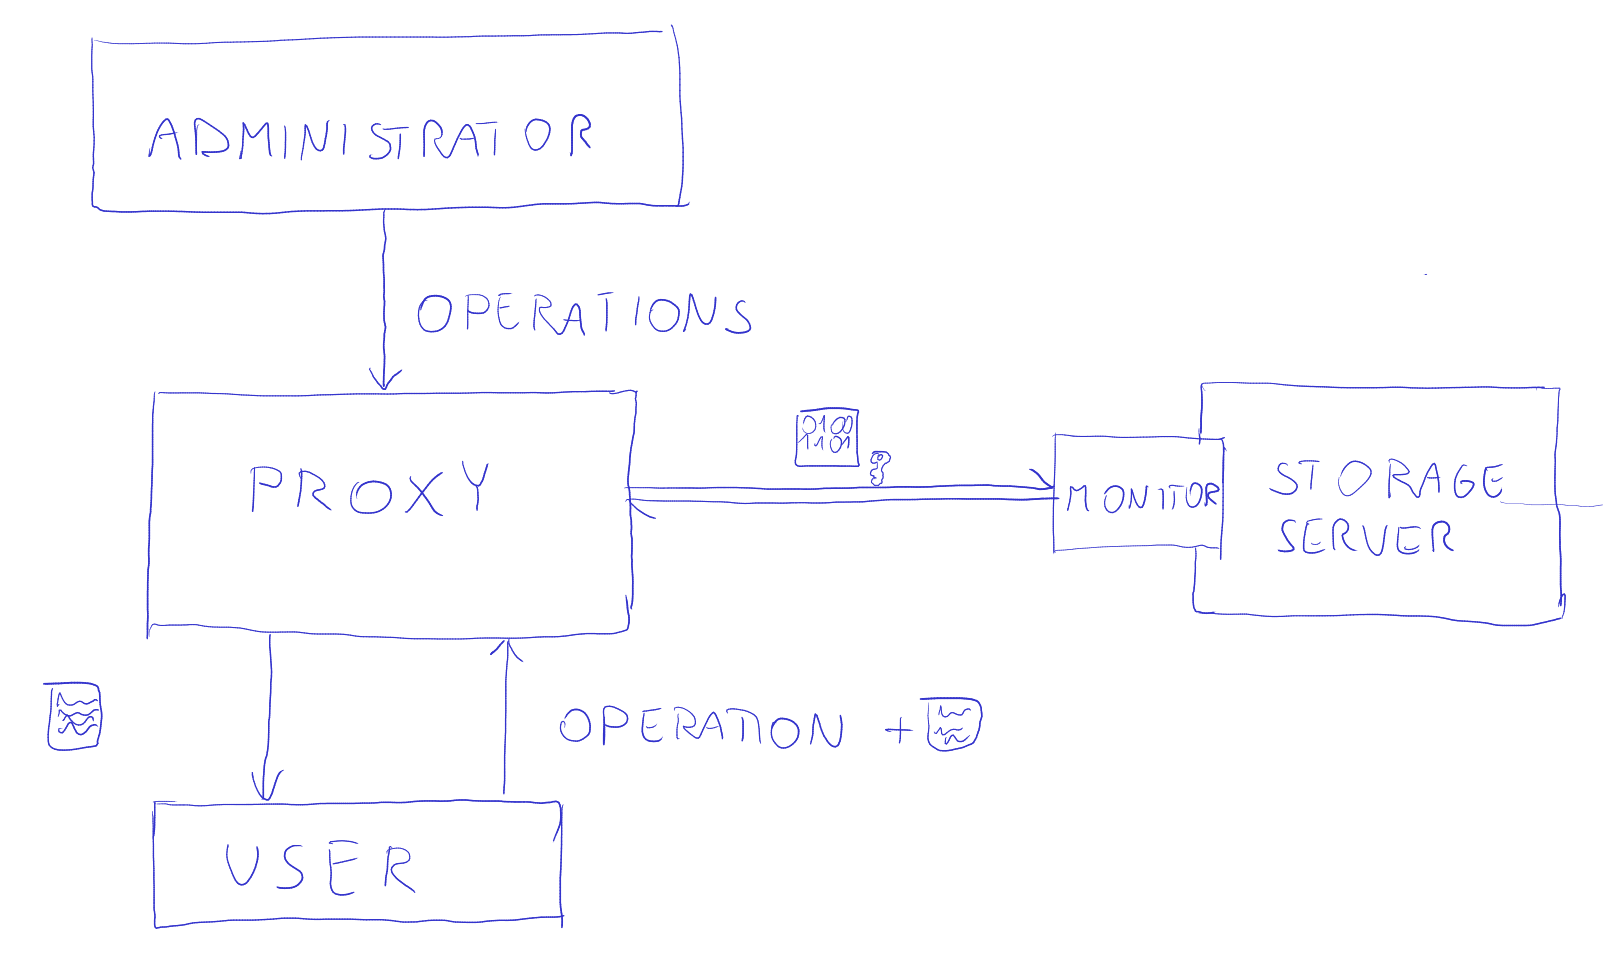
\includegraphics[width=\textwidth]{assets/img/scheme1.png}
		% % 		\caption{Currend scheme}
		% % 		\label{fig:scheme_old}
		% % 	\end{subfigure}
	% % 	\begin{subfigure}{0.48\textwidth}
		% % 		\centering
		
		% % 		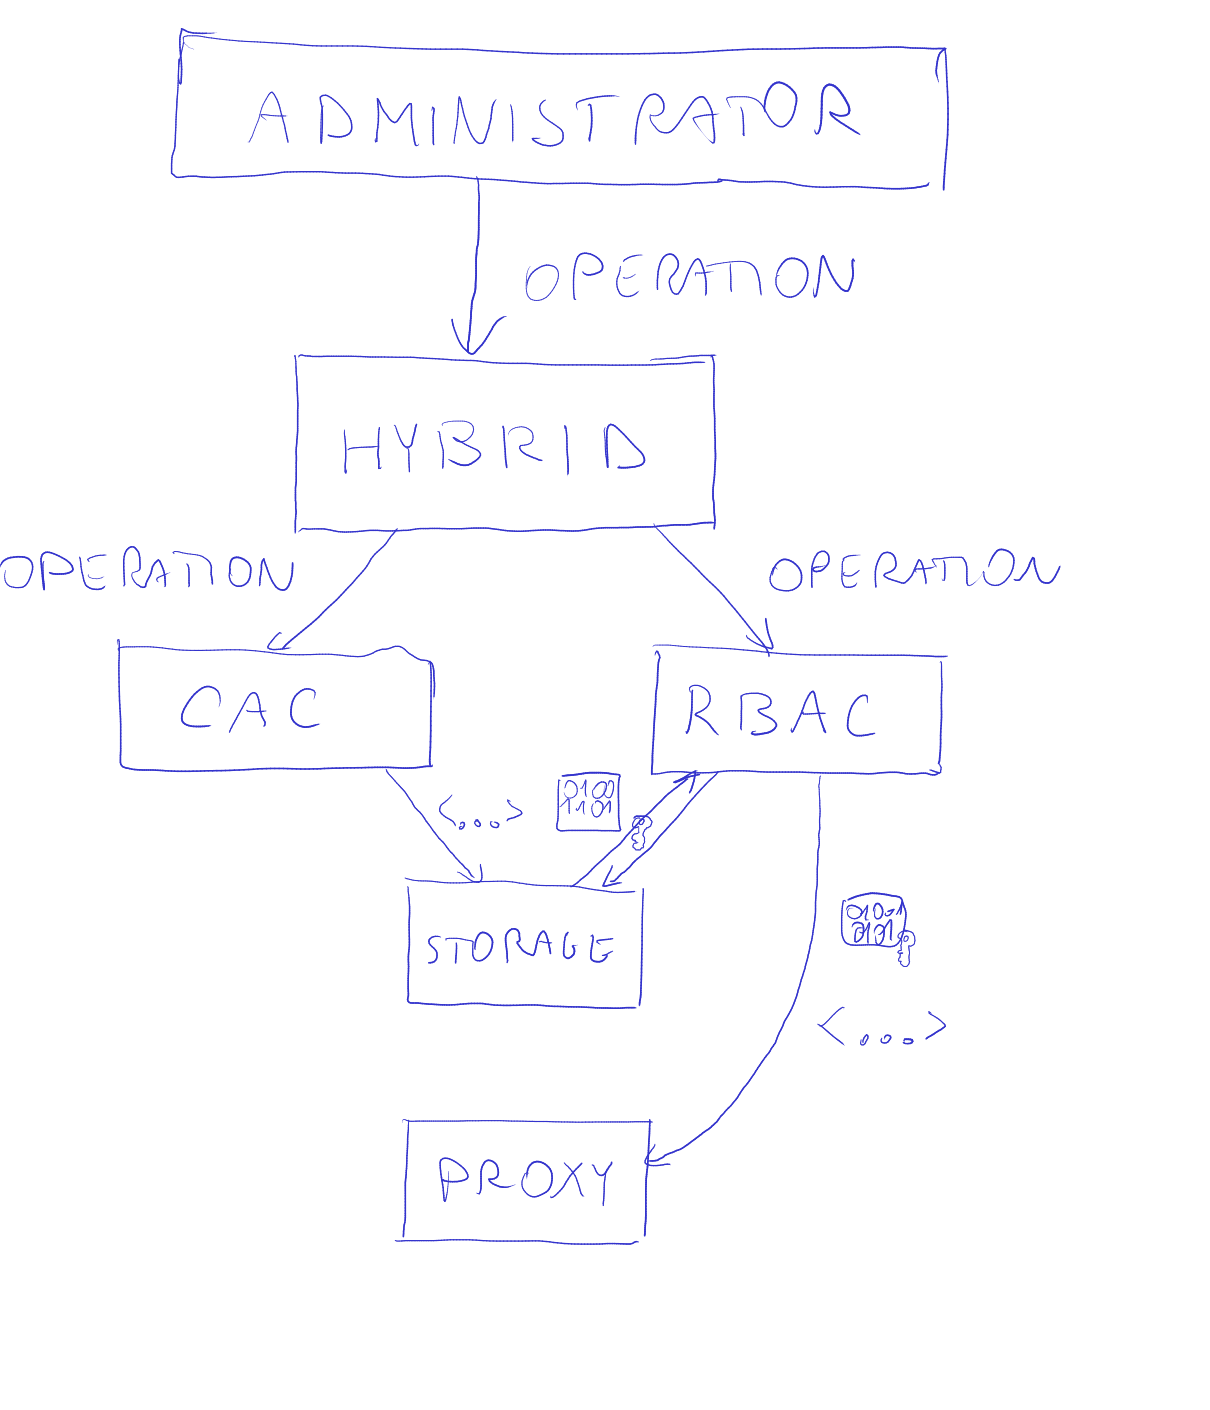
\includegraphics[width=\textwidth]{assets/img/scheme2.png}
		% % 		\caption{Proposed scheme}
		% % 		\label{fig:scheme_prop}
		% % 	\end{subfigure}
	
	% % 	\caption{Current and proposed scheme \simonenote{questa realizzazione di queste immagini mi convince molto poco}}
	% % 	\label{fig:scheme}
	% % \end{figure}


\wraptable{|c|c|X|}{\label{fig:symbols}Symbols}{
    \threecols{\textbf{Category}}
              {\textbf{Symbol}}
              {\textbf{Description}}
    \threecolsnl{\multirow{6}{*}{\acrshort{ac}}}
                {\( \states \)}
                {the set of states}
    \threecolsnl{}
                {\( \state \)}
                {a state, \( \state \in \states \)}
    \threecolsnl{}
                {\( \queries \)}
                {the set of queries}
    \threecolsnl{}
                {\( \entailment \)}
                {the entailment function}
    \threecolsnl{}
                {\( \scrules \)}
                {the state-change rules}
    \threecolsnl{}
                {\( \scrule \)}
                {a state-change rule, \( \scrule \in \scrules \)}
    \hline
    \threecolsnl{\multirow{14}{*}{\acrshort{rbac}}}
                {\( \users \)}
                {the set of users}
    \threecolsnl{}
                {\( \user \)}
                {a user, \( \user \in \users \)}
    \threecolsnl{}
                {\( \roles \)}
                {the set of roles}
    \threecolsnl{}
                {\( \role \)}
                {a role, \( \role \in \roles \)}
    \threecolsnl{}
                {\( \files \)}
                {the set of resources (files)}
    \threecolsnl{}
                {\( \file \)}
                {a resource (file), \( \file \in \files \)}
    \threecolsnl{}
                {\( \urassignement \)}
                {the set of user-role assignments}
    \threecolsnl{}
                {\( \operations \)}
                {the set of operations}
    \threecolsnl{}
                {\( \operation \)}
                {an operation, \( \operation \in \operations \)}
    \threecolsnl{}
                {\( \opread \)}
                {read operation, \( \opread \in \operations \)}
    \threecolsnl{}
                {\( \opwrite \)}
                {write operation, \( \opwrite \in \operations \)}
    \threecolsnl{}
                {\( \opreadwrite \)}
                {both read and write operations}
    \threecolsnl{}
                {\( \permissions \)}
                {the set of all possible permissions}
    \threecolsnl{}
                {\( \frassignement \)}
                {is the permission-role assignement}
    \hline
    \threecolsnl{\multirow{2}{*}{Extended  \gls{rbac}}}
                {\( \predicates \)}
                {the set of predicates}
    \threecolsnl{}
                {\( \prassignement \)}
                {the set of predicate-entity assignement}
    \hline
    \threecolsnl{\multirow{15}{*}{CAC}}
                {\( \genpub \)}
                {generate asymmetric key-pair}
    \threecolsnl{}
                {\( \gensig \)}
                {generate signing key-pair}
    \threecolsnl{}
                {\( \gensym \)}
                {generate symmetric key}
    \threecolsnl{}
                {\( \keyenc{\actor} \)}
                {encryption key of entity \( \actor \)}
    \threecolsnl{}
                {\( \keydec{\actor} \)}
                {decryption key of entity \( \actor \)}
    \threecolsnl{}
                {\( \keysig{\actor} \)}
                {signing key of entity \( \actor \)}
    \threecolsnl{}
                {\( \keyver{\actor} \)}
                {verification key of entity \( \actor \)}
    \threecolsnl{}
                {\( \key{}{\file} \)}
                {encryption key of file \( \file \)}
    \threecolsnl{}
                {\( \encpub{\keyenc{\actor}}{...} \)}
                {encrypt with key \( \keyenc{\actor} \) (asymmetric)}
    \threecolsnl{}
                {\( \decpub{\keyenc{\actor}}{...} \)}
                {decrypt with key \( \keyenc{\actor} \) (asymmetric)} 
    \threecolsnl{}
                {\( \encsym{\keyenc{\actor}}{...} \)}
                {encrypt with key \( \keyenc{\actor} \) (symmetric)}
    \threecolsnl{}
                {\( \decsym{\keyenc{\actor}}{...} \)}
                {decrypt with key \( \keyenc{\actor} \) (symmetric)} 
    \threecolsnl{}
                {\( \sig{\actor} \)}
                {signature made by \( \actor \)}
    \threecolsnl{}
                {\( \verifysig{\key{}{\actor}}{...} \)}
                {verification with the key of \( \actor \)}
    \hline
    \threecolsnl{\multirow{9}{*}{Costs}}
                {\( \cgensig \)}
                {generation of a signing key-pair}
    \threecolsnl{}
                {\( \cgenpub \)}
                {generation of an asymmetric key-pair}
    \threecolsnl{}
                {\( \gensym \)}
                {generation of a symmetric key}
    \threecolsnl{}
                {\( \cencsym \)}
                {encryption with a symmetric algorithm}
    \threecolsnl{}
                {\( \cencpub \)}
                {encryption with an asymmetric algorithm}
    \threecolsnl{}
                {\( \cdecsym \)}
                {decryption with a symmetric algorithm}
    \threecolsnl{}
                {\( \cdecpub \)}
                {decryption with an asymmetric algorithm}
    \threecolsnl{}
                {\( \csig \)}
                {signing data}
    \threecolsnl{}
                {\( \cverifysig \)}
                {verification signed data}
    \hline
}


% \begin{table}
%     \begin{tabularx}{\textwidth}{preamble}
        
%     \end{tabularx}
% \end{table}


% \begin{table}
% 	%	\scriptsize
% 	%	\setlength\tabcolsep{2.0pt}
% 	\caption{Symbols}
% 	\begin{tabularx}{\linewidth}{c|c*1{>{\sloppy\arraybackslash} X }}
		
% 		\hline
		
% 		\multicolumn{1}{c}{Level} &
% 		\multicolumn{1}{c}{Symbol} &
% 		\multicolumn{1}{c}{Description} \\
% 		\hline
		
		
% 		\multirow{4}{*}{Policy} &		
% 		$\policy$ &
% 		The \gls{ac} policy \\
		
% 		% &
% 		% \cellcolor{cloud}$\predicates$ &
% 		% \cellcolor{cloud}The set of predicates \\
		
% 		% &
% 		% $\policyt$ &
% 		% The \gls{ac} policy to enforce traditionally ($\policyt \subseteq \policy$) \\		
		
% 		% &
% 		% \cellcolor{cloud}$\policyc$ &
% 		% \cellcolor{cloud}The \gls{ac} policy to enforce cryptographically ($\policyc \subseteq \policy$) \\
		
% 		% \hline
		
		
		
% 		% \multirow{7}{*}{Model} &
% 		% $\users$ &
% 		% The set of users \\
		
% 		% &
% 		% \cellcolor{cloud}$\roles$ &
% 		% \cellcolor{cloud}The set of roles \\
		
		
% 		% &
% 		% $\files$ &
% 		% The set of files \\	
		
% 		% &
% 		% \cellcolor{cloud}$\operations$ &
% 		% \cellcolor{cloud}The set of operations that can be performed over files \\	
		
		
% 		% &
% 		% $\permissions$ &
% 		% The set of permissions that can be distributed ($\permissions \subseteq \files \times \operations$) \\	
		
% 		% &
% 		% \cellcolor{cloud}$\ur$ &
% 		% \cellcolor{cloud}The set of assignments between users and roles ($\ur \subseteq \users \times \roles$) \\	
		
		
% 		% &
% 		% $\pa$ &
% 		% The set of assignments between roles and permissions ($\pa \subseteq \roles \times \permissions$) \\	
		
% 		% \hline
		
		
		
% 		% \multirow{8}{*}{Enforcement} &
% 		% $\users_{\mm t}$ &
% 		% The set of users' data; each element is a single value $u$ \\
		
% 		% \multirow{8}{*}{(Traditional)} &
% 		% \cellcolor{cloud}$\roles_{\mm t}$ &
% 		% \cellcolor{cloud}The set of roles' data; each element is a single value $r$\\
		
% 		% &
% 		% $\files_{\mm t}$ &
% 		% The set of files' data; each element is a single value $f$\\
		
% 		% &
% 		% \cellcolor{cloud}\multirow{2}{*}{$\operations_{\mm t}$} &
% 		% \cellcolor{cloud}The set of operations that can be performed over files ($\operations_{\mm t} = {\rperm, \wperm}$) \\	
		
% 		% &
% 		% \multirow{2}{*}{$\ur_{\mm t}$} &
% 		% The set of data related to the assignments between users and roles; each element is a tuple $(u,r)$ \\	
		
% 		% &
% 		% \cellcolor{cloud}\multirow{2}{*}{$\pa_{\mm t}$} &
% 		% \cellcolor{cloud}The set of data related to the assignments between roles and permissions; each element is a tuple $(r, \langle f, \mathit{op} \rangle )$ \\	
		
		
		
% 		% \hhline{|~|--|}
		
		
		
% 		% \multirow{16}{*}{Enforcement} &
% 		% $\users_{\mm c}$ &
% 		% The set of users' data; each element is a tuple $(u,\token_u,\enckey_u,\verkey_u)$ \\
		
% 		% \multirow{16}{*}{(Cryptographic)} &
% 		% \multirow{2.5}{*}{\cellcolor{cloud}$\roles_{\mm c}$} &
% 		% \cellcolor{cloud}The set of roles' data; each element is a tuple $(r,\token_{(r,v_r)},\enckey_{(r,v_r)},\verkey_{(r,v_r)}, v_r)$ \\
		
% 		% &
% 		% $\files_{\mm c}$ &
% 		% The set of files' data; each element is a tuple $(f, \token_{(f,v_f)}, v_f)$ \\
		
% 		% &
% 		% \cellcolor{cloud}\multirow{2}{*}{$\operations_{\mm c}$} &
% 		% \cellcolor{cloud}The set of operations that can be performed over files ($\operations_{\mm c} = {\rperm, \wperm}$) \\	
		
% 		% &
% 		% \multirow{3.5}{*}{$\roletuples$} &
% 		% The set of data related to the assignments between users and roles; each element is a tuple $(u,r,\PKEnc_{\enckey_{u}}\left( \enckey_{(r,v_r)}, \deckey_{(r,v_r)}, \verkey_{(r,v_r)}, \sigkey_{(r,v_r)} \right), v_r)$ \\	
		
% 		% &
% 		% \cellcolor{cloud}\multirow{3.5}{*}{$\permissiontuples$} &
% 		% \cellcolor{cloud}The set of data related to the assignments between roles and permissions; each element is a tuple $(r, f, \token_{(r,v_r)}, \token_{(f,v_f)}, \PKEnc_{\enckey_{(r,v_r)}}\left( \symkey_{(f,v_f)} \right), v_r, v_A, \mathit{op})$ \\
		
% 		% &
% 		% \multirow{2}{*}{$\filetuples$} &
% 		% The set of data related to encryption types and file version numbers; each element is a tuple $(f, \token_{(f,v_f)}, v_f, \encType_f, \token_{(r,v_r)})$ \\ 
		
% 		% &
% 		% \cellcolor{cloud}\multirow{2}{*}{$\roleshadowgroup$} &
% 		% \cellcolor{cloud}The set of data related to the assignments between roles and shadow groups; each element is a tuple $(r,g)$\\		
		
		
		
% 		% \bottomrule
		
% 	\end{tabularx}
% 	\label{table:notation}
% \end{table}


